\documentclass{article}
\usepackage[ansinew]{inputenc}
\usepackage{lmodern}
\usepackage[T1]{fontenc}
\usepackage[spanish,activeacute]{babel}
\usepackage{mathtools}
\usepackage{graphicx}
\usepackage{float}
\usepackage[dvipsnames]{xcolor}
\usepackage{textcomp}
\definecolor{Mycolor1}{HTML}{008000}

\title{Treball Final de M�ster}
\author{Josep Maria Mart� }
\date{February 2017}

\begin{document}

\maketitle
\newpage
\section{Easy Driver A3967}

Per facilitar el control dels motors pas a pas utilitzats, s\textquotesingle ha decidit utilitzar dos controladors Easy Driver A3967 que facilitar� el control i la programaci� dels motors i actuara com etapa de pot�ncia per no sobrecarregar l\textquotesingle Arduino amb la potencia requerida pel motor.
\\*
\\*
Com ja s\textquotesingle ha explicat, els motors pas a pas funcionen amb el canvi d\textquotesingle excitaci� de les bobines que el conformen, i cada parell de bobines te el seu parell de cables per fer-ho. La idea principal d\textquotesingle aquest driver o controlador �s facilitar la feina i encarregar-se de l\textquotesingle alimentaci� dels motors, permetent aix� a l\textquotesingle usuari controlar el motor a trav�s de nom�s dos pins digitals de l\textquotesingle Arduino, l\textquotesingle STEP, que defineix un pas per cada pujada del pin i el DIR, que defineix el sentit de rotaci� del motor. 
\\*
\\*
A la seg�ent imatge es mostra la distribuci� de les diferents entrades amb les que compta el controlador:

\begin{figure}[h]
	\centering
		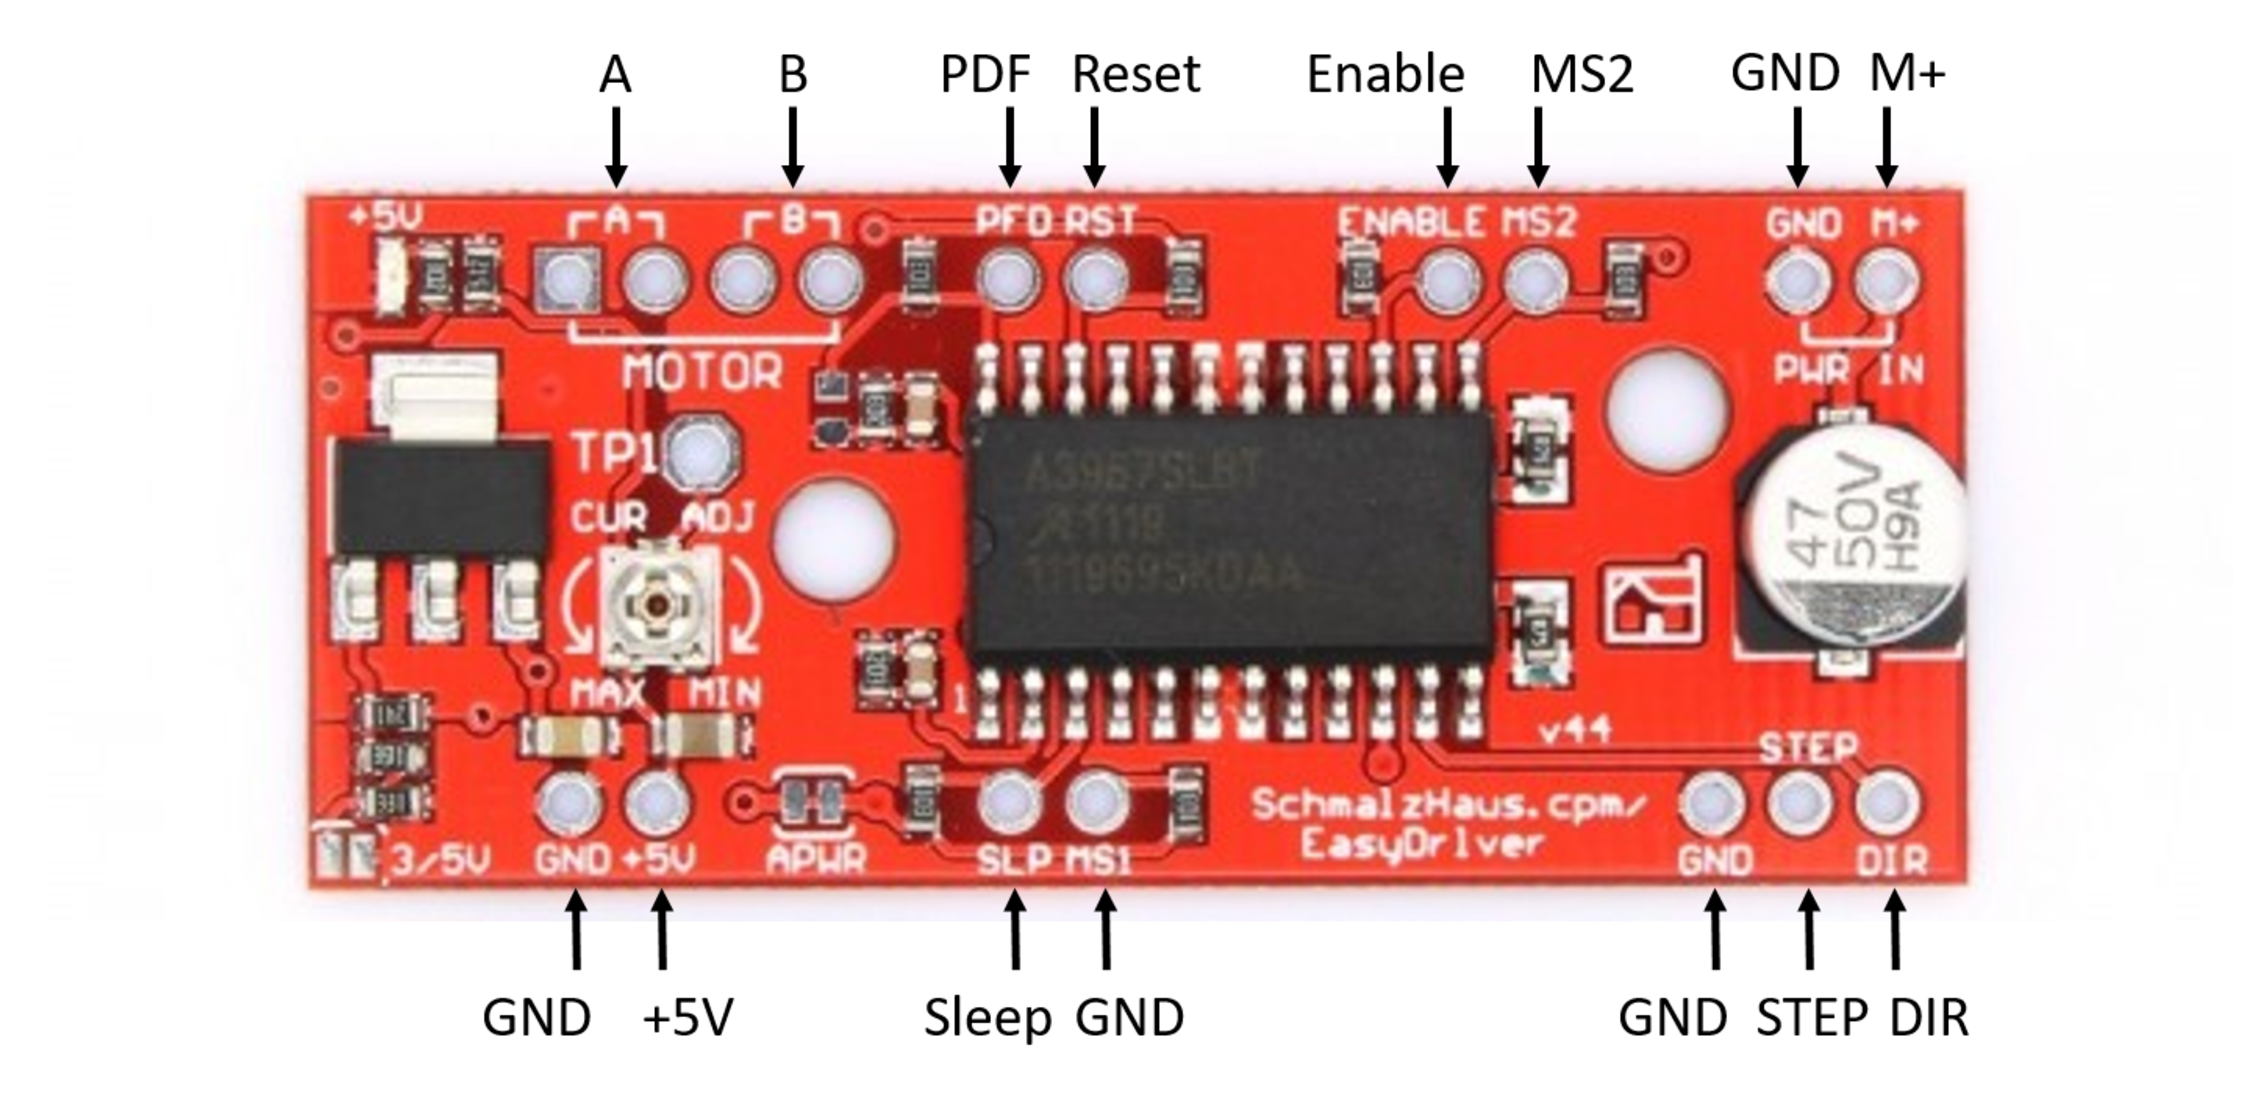
\includegraphics[width=1.00\textwidth]{C:/Users/usuario/Documents/GitHub/TFM/PinsA3967.eps}
	\caption{Figura 1. Pins del driver A3967.}
	\label{fig:PinsA3967}
\end{figure}


Els pins principals i imprescindibles s�n els seg�ents:


\begin{itemize}

\item	A i B: Aquestes son les entrades dels 4 cables del motor, s\textquotesingle ha de connectar tenint en compte els dos parells de bobines diferents, una al als pins A i l\textquotesingle altre als pins B. L\textquotesingle ordre dels cables del mateix parell de bobines �s indiferent.

\item GND: Hi ha tres pins amb aquest nom i s�n la connexi� a terra necess�ria a qualsevol circuit electr�nic.

\item STEP: Connectat a un pin digital d\textquotesingle Arduino, es l\textquotesingle encarregat de realitzar els passos del motor. A cada pujada de 0 a 5V, ordena al motor realitzar un pas. 

\item DIR: Igual que l\textquotesingle STEP, va connectat a un pin digital d\textquotesingle Arduino (0-5V) i defineix segon el seu estat (high/low) la direcci� del motor.

\item M+: �s l\textquotesingle entrada positiva de la font d\textquotesingle alimentaci� del motor i es recomana alimentar-la a un m�xim de 12V. L\textquotesingle entrada negativa de la font es connecta al pin GND del costat.

\end{itemize}

La resta de pins permeten modificar el comportament del motor, per� s�n opcionals:

\begin{itemize}

\item MS1 i MS2: Aquests pins s�n els encarregats del microstepping. Poden reduir l\textquotesingle angle del pas i per tant augmentar la precisi� de moviment del robot ja que redueixen moviment per pas. Hi ha 4 opcions de funcionament en funci� de la connexi� d\textquotesingle aquests dos pins que poden ser 0V (low) o 5V (high). El pas normal o full-step s\textquotesingle aconsegueix amb la combinaci� low/low, el mig pas o half-step amb high/low, un quart de pas o quarter-step amb low/high i un vuit� de pas o eight-step amb high/high. Per defecte la connexi� �s high/high, i per tant divideix el pas per 8. 

\item Enable: �s un input connectat com a low que elimina les sortides si es canvia a high.

\item Reset: �s un input connectat com a high que quan es canvia a low torna el controlador a la configuraci� inicial. 

\item Sleep: �s un input connectat com a high que minimitza el consum dels motors quan aquests no s\textquotesingle utilitzen si es canvia a low.

\item +5V: Output de 5V que es pot utilitzar per alimentar components que funcionin a baixa corrent. 

\item PDF: Aquest pin no s\textquotesingle utilitza, controla el mode de decad�ncia del corrent de sortida.

\end{itemize}

\end{document}